% ----------------- CHAPTER 1 -----------------
\pagenumbering{arabic}
\chapter{Introduction}

\indent
Deep neural networks (DNNs) have achieved remarkable success in image classification tasks~\cite{he2016deep, krizhevsky2012imagenet}. However, they remain vulnerable to \emph{adversarial examples} which are the inputs with imperceptibly small perturbations that cause misclassification~\cite{szegedy2013intriguing, goodfellow2014explaining}, raising concerns for safety-critical applications such as autonomous driving~\cite{Eykholt_2018_CVPR} and facial recognition~\cite{sharif2016accessorize}.

\begin{figure}[htbp]
    \centering
    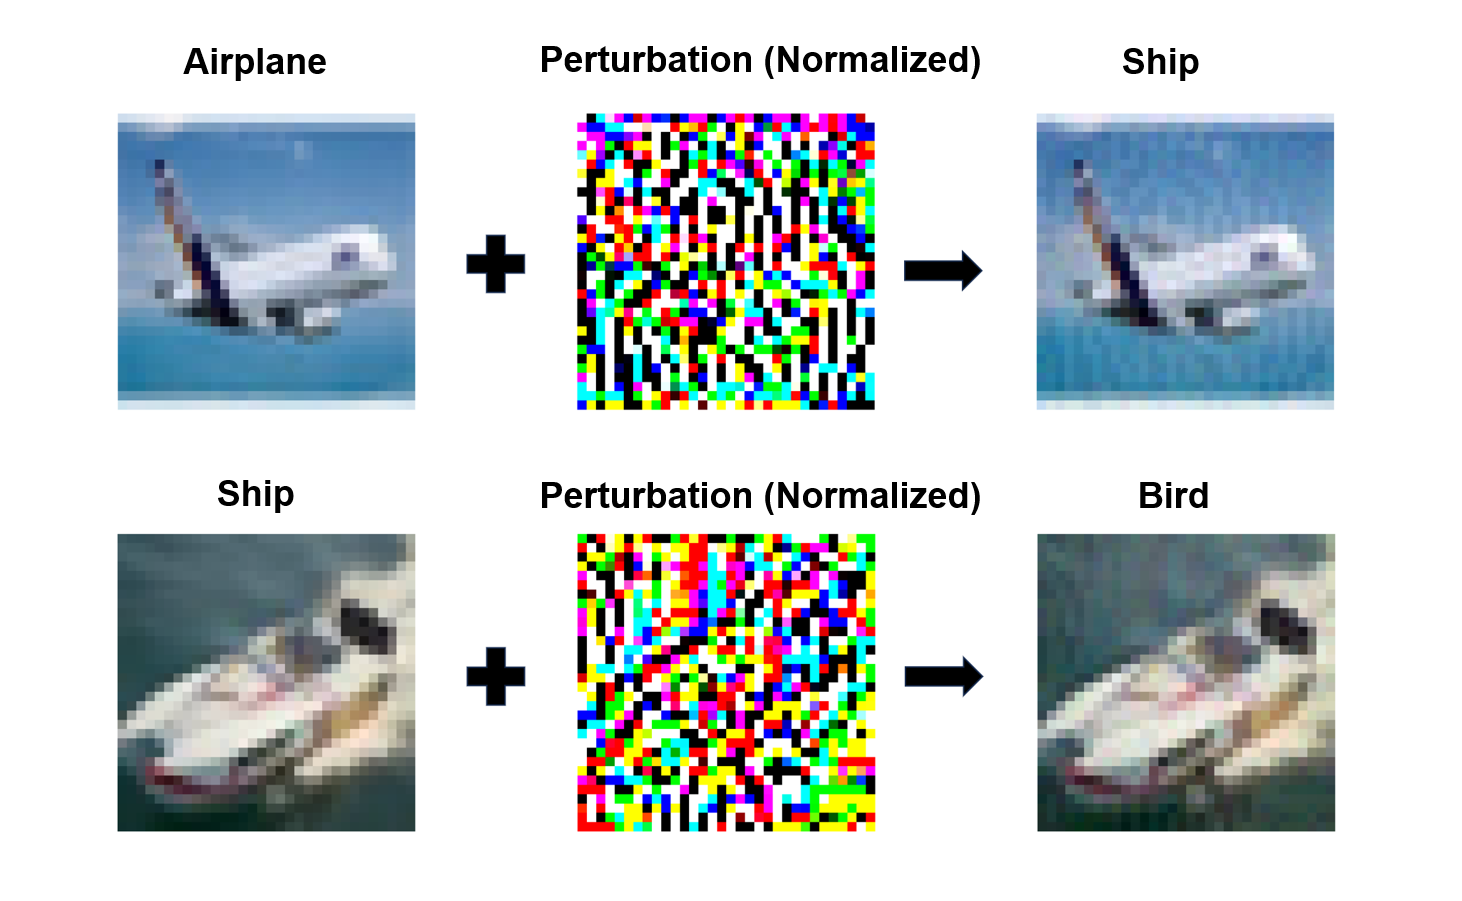
\includegraphics[width=0.85\linewidth]{images/Adversarial examples.png}
    \caption{Adversarial examples on CIFAR-10. Each row shows the original image with true label(left), the perturbation (middle), and the adversarial image with isclassification (right).}

    \label{fig:adv_examples}
\end{figure}

To address these threats, a wide range of adversarial defense strategies have been proposed. A comprehensive systematization of certified robustness techniques was provided by Li et al.~\cite{li2023sok}, who categorized existing methods into verification-based approaches (e.g., LP~\cite{wong2018provable} and MILP~\cite{tjeng2017evaluating}) and training-based approaches (e.g., robust training with bound propagation~\cite{gowal2018effectiveness}). This work also highlights the trade-offs between the quality of computed certified bounds and scalability. 
Certified defenses~\cite{cohen2019certified, gowal2018effectiveness} provide provable guarantees against norm-bounded attacks (e.g., $\ell_\infty$), but often suffer from scalability and computational cost. In contrast, empirical defenses, such as adversarial training~\cite{madry2017towards, wong2020fast} are more scalable and effective in practice but can remain susceptible to adaptive or unforeseen attacks~\cite{tramer2020adaptive}.


This project builds on both certified and empirical perspectives. In particular, we investigate certified training methods such as the LP-based training proposed by Wong and Kolter~\cite{wong2018provable}, alongside empirical defenses.

Among empirical approaches, ensemble-based defenses have emerged as a promising direction for enhancing robustness. By aggregating predictions from multiple models, ensembles can potentially mitigate the vulnerabilities of individual models and improve overall reliability~\cite{abbasi2017robustness, pang2019improving}. Traditional ensemble methods, such as majority voting or logits averaging, have shown some improvement in robustness, but they often lack a principled way to assess prediction confidence, making it difficult to determine whether the ensemble’s output is reliable under adversarial conditions.


Recently, \textit{CrossMax} was introduced as part of the ``Ensemble Everything Everywhere'' framework~\cite{fort2024ensemble}, providing a robust aggregation mechanism for ensemble predictions. We expand on the original design: Traditional ensemble methods, such as averaging logits or probabilities, are susceptible to attacks targeting a single model, where an outlier prediction can dominate the aggregate output. CrossMax mitigates this by drawing inspiration from Vickrey auctions: it considers each model as a bidder and aggregates predictions using the $k$-th largest logits per class rather than the maximum. Additional normalization steps, including subtracting each predictor's maximum and the per-class maximum, prevent individual models or classes from dominating spuriously. This dynamic aggregation ensures that the ensemble's decision reflects consistent agreement across models, enhancing robustness against targeted adversarial perturbations.


However, subsequent work~\cite{zhang2024evaluating} challenged these findings, attributing the apparent robustness gains largely to \textit{gradient masking}, a known evaluation pitfall. They showed that attacking the \textit{mean aggregation} mechanism and evaluating CrossMax yields stronger adversarial examples than directly attacking CrossMax itself, suggesting that CrossMax impedes gradient-based optimization rather than offering true robustness improvements.


Despite this criticism, CrossMax retains robustness benefits by leveraging model disagreement. Prior works focused solely on \textit{single-label predictions}. In contrast, we highlight a novel property: \textbf{CrossMax can produce multi-label prediction sets with a bounded size}, as detailed in Appendix~\ref{appendix:crossmax-bound}. The proportion of samples with single-label predictions, i.e., prediction sets of size one, serves as a proxy for ensemble confidence under attack. Our experiments reveal that ensembles of robustly trained models maintain a more stable single-label prediction rate compared to naturally trained ones, offering a new perspective on interpreting ensemble confidence and robustness beyond standard accuracy metrics.


The contributions of this work are threefold. First, we provide a comprehensive empirical evaluation of ensemble defense methods against strong white-box adversarial attacks, including APGD, FABAttack\_PT, and targeted APGD, as well as the query-based black-box SquareAttack~\cite{croce2020reliable}, highlighting their robustness performance under varying perturbation budgets. Second, we systematically study the effects of architectural diversity and training perturbation budgets on ensemble robustness, revealing important trade-offs and insights. Third, we analyze ensemble confidence behaviors across multiple aggregation strategies, with a particular focus on CrossMax, elucidating its strengths as well as limitations in practical robustness scenarios.

Through these contributions, we offer new insights into how ensemble methods, especially CrossMax, can effectively bridge the gap between certified robustness guarantees and empirical adversarial resilience, balancing robustness with clean accuracy. The code and implementation details for this project are available at our GitHub repository: https://github.com/samavi/lpsdp.git
